\def\VCDate{2016/03/08}\def\VCVersion{(Current)}
\documentclass{article}
\usepackage{ProofPower,verbatim,graphicx,float}
\usepackage{amsmath,amsfonts}
\usepackage{underscore,listings}
\usepackage[margin=0.5in,paperwidth=6in,paperheight=5in]{geometry}
\title{gcd function in sml, C, and asm}
\setcounter{secnumdepth}{0}
\begin{document} 
\maketitle
\tableofcontents
\clearpage\section{gcd}
The greatest common divisor (gcd) of two positive natural numbers is the largest natural 
number that exactly divides both numbers. 
The gcd of 14 and 12 is 2, while the gcd of 14 and 11 is 1.
The gcd is given by this specification:
\[ \text{gcd} : (\mathbb{N} \times \mathbb{N}) \rightarrow \mathbb{N} \]
\[ \text{gcd}(m,n) = \text{max}\{d \in \mathbb{N} \vert m \bmod d = 0 \land n \bmod d = 0\} \]

One {\it algorithm} for calculating the gcd follows Euclid's method. If, for two positive natural
numbers $m$ and $n$, we have that $m>n$, then the gcd of $m$ and $n$ is defined by:
\[ \text{euclid} : (\mathbb{N} \times \mathbb{N}) \rightarrow \mathbb{N} \]
\[ \text{euclid}(m,n) = 
     \left\{
        \begin{array}{lr}
             \text{euclid}(n,m \bmod n), & \text{if} \; n > 0 \\
             m, & \text{otherwise}
        \end{array}
      \right.
 \]
\clearpage\section{gcd in sml}
This can be written in SML like this:
\begin{GFT}{SML}
\+fun euclid m n = if n > 0\\
\+                    then euclid n (m mod n)\\
\+                    else m ;\\
\+euclid 558 198;  (* expect 18 *)\\
\end{GFT}
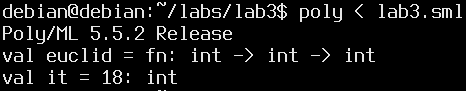
\includegraphics[scale=0.5]{fig1.png}\\

Although a short program, we may not be familiar with the use of recursion because it is not commonly used for C programs due to its inefficiency. But let's implement it that way anyway to follow the math definition more closely.
\clearpage\section{gcd in c}
\begin{GFT}{C source code written to file lab3.c}
\+\#include <stdio.h>\\
\+int euclid(int m, int n)\\
\+\{\\
\+  if( n > 0) return euclid(n, m \% n);\\
\+  else return m;\\
\+\}\\
\+int main()\\
\+\{\\
\+  printf("\%i\Backslash{}n",euclid(558,198));\\
\+  return 0;\\
\+\}\\
\+\\
\end{GFT}
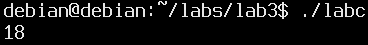
\includegraphics[scale=0.5]{fig2.png}
\clearpage
The first line of this C code is an include to get access to the library. We need it here to use printf.
\lstinputlisting[language=C,linerange={1-1}]{lab.c}
In ASM, we do not need to include any files in order to link to the C library, so we can skip this.
\clearpage\subsection{gcd in c: euclid function}
\lstinputlisting[language=C,linerange={2-6}]{lab.c}
These lines are the function definition. There are several techniques to be studied to implement it in assembler:
\begin{itemize}
\item syntax for function definitions
\item parameter passing
\item decision (if statement)
\item conditional (relational expression to compare values)
\item return statement
\item calling a function (recursively in this case)
\item calculating modulus
\end{itemize}

\clearpage\subsection{gcd in asm: main}
%\lstinputlisting[language=C,linerange={7-11}]{lab.c}
The main function is simpler, but we need to also learn how to: 
\begin{itemize}
\item call printf
\item end the program
\end{itemize}
ASM code is put in the ``text'' section. The entry point is named ``_start''. It is a label (indicated by the colon). We make it global so the linker will make it visible to be called externally (by the operating system).
\begin{GFT}{ASM source code written to file lab3.s}
\+.text\\
\+.globl \_start\\
\+\_start:\\
\+\\
\end{GFT}
\clearpage
printf needs 2 parameters: a format string and a value. That value must be determined by called our function euclid. Return values are found in the EAX register. The euclid function also requires 2 parameters which must be pushed onto the system stack so they can be retrieved within the function. Parameters are pushed right to left (the C convention). Immediate (literal) values are prefixed with the \$ sign. Register names are prefixed with the \% sign.
\begin{GFT}{ASM source code appended to file lab3.s}
\+push \$198\\
\+push \$558\\
\+call euclid\\
\+add \$8, \%esp \#two of them 4 bytes each\\
\+.data\\
\+fmt: .string "\%i\Backslash{}n"\\
\+.text\\
\+push \%eax\\
\+push \$fmt\\
\+call printf\\
\+add \$8, \%esp\\
\+\\
\end{GFT}
\clearpage
The program is ended by calling software interrupt 0x80. The 1 in EAX means exit command and the 0 in EBX is the convention to mean program had no errors.
\begin{GFT}{ASM source code appended to file lab.s}
\end{GFT}
\clearpage\subsection{gcd in asm: euclid function}
The euclid function uses the same technique of creating a label to indicate start of function. It ends with the ret instruction. The first 2 instructions set up a stack frame base pointer (EBP) to give us access to paramters even if the stack pointer (ESP) moves.
\begin{GFT}{ASM source code appended to file lab.s}
\end{GFT}
Now we can access the 2 parameters using register EBP. 4 bytes above EBP is the return address, 8 is the 1st parm, and 12 is the second. i.e.
\begin{description}
\item[n] is on stack at \verb|12(%ebp)|
\item[m] is on stack at \verb| 8(%ebp)|
\end{description}
The if statement has to be simulated by branching to labels depending of results of doing the comparison of n to zero.
\begin{GFT}{ASM source code appended to file lab.s}
\end{GFT}
This is the ``then'' part of the if statement. We need to calculate $m \mod n$ and call euclid again!  Integer division is done by putting dividend in EDX:EAX as 64-bit value, and divisor in EBX. The remainder will be in EDX.
\begin{GFT}{ASM source code appended to file lab3.s}
\end{GFT}
\clearpage
These last 2 instructions undo the first 2--they restore the original stack as it was found on entry to the function.
\begin{GFT}{ASM source code appended to file lab3.s}
\end{GFT}
Here is output from running the ASM program:\\
%\includegraphics[scale=0.8]{fig3.png}\\
\clearpage
\begin{GFT}{Text written to file labcode.sh}
\+docsml lab.doc\\
\+as -gstabs -o lab.o lab.s\\
\+ld -dynamic-linker /lib/ld-linux.so.2 -o labasm lab.o -lc -lX11\\
\+gcc -o labc lab3.c\\
\end{GFT}
\begin{GFT}{Text written to file labdoc.sh}
\+doctex lab3.doc\\
\+pptexenv /home/debian/texfot.pl pdflatex lab3.tex\\
\end{GFT}
\begin{GFT}{Bourne Shell}
\+chmod 755 labcode.sh\\
\+chmod 755 labdoc.sh\\
\end{GFT}
\end{document}

